\documentclass[11pt,a4paper]{article}

\usepackage[utf8]{inputenc}
\usepackage[T1]{fontenc}
\usepackage{lmodern}
\usepackage[margin=2.3cm]{geometry}
\usepackage{microtype}
\usepackage{amsmath,amssymb}
\usepackage{booktabs}
\usepackage{tabularx}
\usepackage{array}
\usepackage{enumitem}
\usepackage{xcolor}
\usepackage{listings}
\usepackage{tikz}
\usetikzlibrary{positioning,arrows.meta,shapes.geometric}
\usepackage[hidelinks]{hyperref}
\usepackage{xurl}

\DeclareUrlCommand\code{\urlstyle{tt}}
\newcolumntype{L}{>{\raggedright\arraybackslash}X}
\newcolumntype{P}[1]{>{\raggedright\arraybackslash}p{#1}}
\setlist{itemsep=2pt,topsep=4pt}

\definecolor{kw}{RGB}{0,70,160}
\definecolor{cm}{RGB}{100,110,100}
\definecolor{st}{RGB}{160,40,40}
\definecolor{bgc}{RGB}{247,247,247}

\lstdefinelanguage{Solidity}{
  morekeywords={pragma,contract,function,returns,return,uint256,uint64,uint32,uint16,uint8,int256,bytes32,bytes4,bytes,bool,address,memory,calldata,storage,public,external,internal,view,pure,payable,struct,mapping,emit,event,require,revert,if,else,for,true,false,abi,keccak256,blockhash,block,msg},
  sensitive=true,
  morecomment=[l]{//},
  morecomment=[s]{/*}{*/},
  morestring=[b]"
}
\lstset{
  basicstyle=\ttfamily\small,
  keywordstyle=\color{kw}\bfseries,
  commentstyle=\color{cm}\itshape,
  stringstyle=\color{st},
  backgroundcolor=\color{bgc},
  frame=single, rulecolor=\color{black!20},
  breaklines=true, breakatwhitespace=false,
  columns=fullflexible, keepspaces=true,
  showstringspaces=false,
  xleftmargin=4pt, xrightmargin=4pt, aboveskip=8pt, belowskip=8pt
}

\newenvironment{deepdive}[1]{\subsection*{Deep dive: #1}\addcontentsline{toc}{subsection}{Deep dive: #1}}{}

\title{\textbf{Arc VRF}\\[4pt]\large Provable randomness for Circle's Arc chain, modelled on Chainlink VRF v2.5\\[2pt]\normalsize Plan \& White Paper}
\author{Himanshu Malik}
\date{Research snapshot: 22 November 2026 (IST)}

\begin{document}
\maketitle

\begin{abstract}
\noindent Smart contracts can't make fair random numbers on their own, and on Arc the usual source (\code{PREVRANDAO}) always returns 0. Arc VRF fixes that. An off-chain service holds a secret key, turns each request into exactly one random number, and attaches a mathematical proof. The Arc VRF contract checks the proof on-chain before your contract ever sees the number.
\begin{enumerate}[label=\arabic*.,leftmargin=1.5em]
  \item \textbf{Pay.} Either fund a subscription once with USDC (subscription method), or send USDC with each request (direct funding).
  \item \textbf{Ask.} Your contract asks the Arc VRF coordinator for $N$ random numbers.
  \item \textbf{Prove.} The Arc VRF node mixes your request with the hash of the block it landed in, runs it through its secret key, and sends back a proof.
  \item \textbf{Check.} The coordinator verifies the proof on-chain. A wrong or invented number fails the check and the transaction reverts.
  \item \textbf{Deliver and bill.} Your contract receives the numbers through a callback, and the fee is charged in USDC.
\end{enumerate}
\end{abstract}

\noindent\small Every fact links to a source read on 22 Nov 2026, or to an on-chain read made that day. Design choices are marked \textbf{[Design choice]}, recommendations \textbf{[Recommendation]}, and anything unchecked \textbf{[Unverified]}. Sections titled \emph{Deep dive} hold technical detail and can be skipped on a first read. ``CL'' refers to \code{smartcontractkit/chainlink-evm} at commit \code{e162754ee3348c8c44a691669f710a06761dd67f}, path \code{contracts/src/v0.8/vrf/} \cite{clcode}.\normalsize

\tableofcontents
\newpage

%-------------------------------------------------------------
\section{Jargon, explained once}
\begin{description}[leftmargin=1em,style=nextline]
  \item[VRF (Verifiable Random Function)] Like a keyed hash where only the key holder can compute the output, but anyone with the public key can verify it \cite{rfc9381}.
  \item[Coordinator] The main on-chain contract. It holds subscriptions, records requests, verifies proofs and pays out results.
  \item[Consumer] Your contract that asks for and receives random numbers.
  \item[Subscription] An on-chain account with a USDC balance and a list of consumers allowed to spend it.
  \item[Wrapper] A contract that lets a consumer pay per request instead of keeping a subscription (direct funding).
  \item[Node / oracle] The off-chain Arc VRF service that watches for requests and submits proofs.
  \item[keyHash / gas lane] Hash of the node's public key; it also sets the maximum gas price you'll pay for fulfilment.
  \item[Callback] The function the coordinator calls on your contract to hand over the numbers (\code{fulfillRandomWords}).
  \item[Block confirmations] How many blocks the node waits before answering, to guard against chain rewrites. Arc has none, so 0 is safe.
  \item[EOA] Externally owned account, an ordinary wallet.
\end{description}

%-------------------------------------------------------------
\section{Overview and key findings}
\begin{itemize}
  \item \textbf{Arc needs this.} Arc's docs say \code{PREVRANDAO} ``always returns 0'' and to use an oracle or VRF instead \cite{arcevm}. Checked on-chain on mainnet and testnet.
  \item \textbf{Chainlink VRF is not on Arc.} Arc is missing from Chainlink's supported-networks page \cite{clnetworks}, and Arc's oracle page lists Chainlink only for Data Feeds and Data Streams \cite{arcoracles}.
  \item \textbf{One VRF is already live on Arc: D20DAO.} Pay per request in USDC, no subscriptions, no consumer allowlist \cite{d20dao}. Arc VRF's subscriptions are the differentiator; its wrapper covers the same pay-per-request case.
  \item \textbf{Both Chainlink payment methods ship in the first release:} subscriptions and direct funding.
  \item \textbf{v2.5 is the version to copy.} VRF v1 shut down on 18 Nov 2026 and v2 shuts down on 30 Nov 2026 \cite{clvrf,clmigv2,clmigv1}.
  \item \textbf{License.} Every Chainlink VRF v2.5 contract file says MIT, but the npm package \code{@chainlink/contracts} declares BUSL-1.1 at package level \cite{cllicense,clnpm}. Forking looks allowed; get a short legal review and never use the Chainlink name. Not legal advice.
  \item \textbf{Deployment target.} Arc testnet first (chain ID 5042002), then Arc mainnet (5042) \cite{arcrpc}.
  \item \textbf{Starting point.} When this paper was written (22 Nov 2026), the repository \code{HimanshuM685/arc-vrf} held only a README, so the plan started from zero \cite{repoarc}. The code now lives in the same repository.
\end{itemize}

%-------------------------------------------------------------
\section{Two ways to pay}
\begin{table}[ht]
\centering\small
\begin{tabularx}{\textwidth}{P{2.8cm}LL}
\toprule
 & \textbf{Subscription} & \textbf{Direct funding}\\
\midrule
Who pays & A subscription balance, charged after each fulfilment & Your contract, paying the wrapper at request time\\
Setup & Create subscription, fund it, add your contracts & Send USDC to your contract; nothing else\\
Contract inherits & \code{ArcVRFConsumerBase} & \code{ArcVRFWrapperConsumerBase}\\
Price & Gas actually used + premium & Callback limit + fixed overheads + premium, quoted up front\\
Limits (Chainlink values) & 100 consumers per subscription, 500 words per request & 10 words per request on Base Sepolia; smaller gas limit\\
Dashboard & Subscription manager & Fee calculator, wrapper settings, request history\\
Best for & Regular requests, several contracts, lower cost per request & Occasional or one-off requests, or end users paying per request\\
\bottomrule
\end{tabularx}
\caption{The two payment methods. Mirrors Chainlink's guidance \cite{clsub,cldf}.}
\end{table}

%-------------------------------------------------------------
\section{Flow 1: Subscription}
The numbers match Chainlink's subscription diagram \cite{clsub}. Everything is on-chain; the dashboard only sends these transactions.

\begin{enumerate}[label=\textbf{\arabic*.}]
  \item \textbf{Set up the subscription.} From your wallet: create a subscription (you get an ID), fund it with USDC, and add the contracts allowed to use it. Order doesn't matter.
  \item \textbf{Use your app.} A user or your wallet calls your contract and pays normal gas.
  \item \textbf{Request.} Your contract calls \code{requestRandomWords} on the coordinator with its subscription ID.
  \item \textbf{Event.} The coordinator records the request and emits \code{RandomWordsRequested}.
  \item \textbf{Wait.} The node waits the requested number of blocks. On Arc this defaults to 0.
  \item \textbf{Respond.} The node submits the proof and pays the gas for that transaction.
  \item \textbf{Deliver.} The coordinator calls your contract's callback with the numbers.
  \begin{enumerate}[label=\textbf{7\alph*.}]
    \item \textbf{LINK conversion:} Chainlink converts gas costs to LINK here. Arc VRF drops this step.
    \item \textbf{Verify and charge:} the proof is checked before delivery; the subscription is charged in USDC (gas used + premium) after it.
  \end{enumerate}
\end{enumerate}

\begin{figure}[ht]
\centering
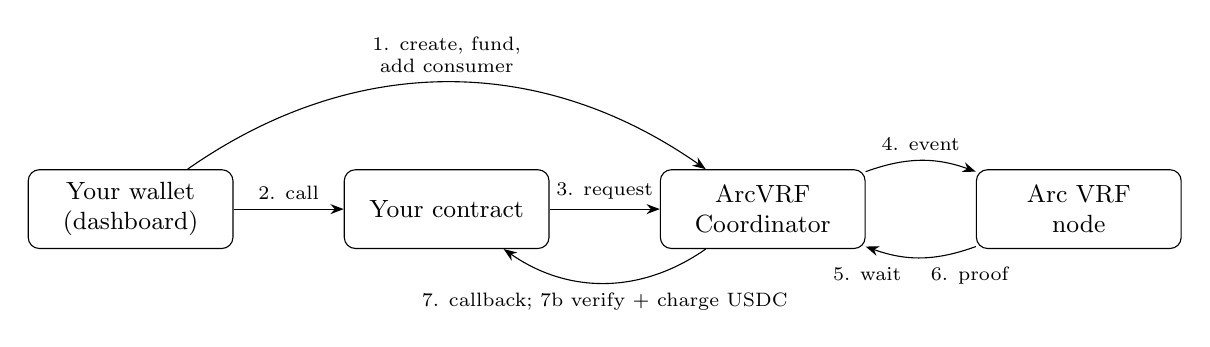
\begin{tikzpicture}[
  box/.style={draw,rounded corners,align=center,minimum width=2.6cm,minimum height=1cm,font=\small},
  lab/.style={font=\scriptsize,align=center},
  >=Stealth]
\node[box] (w) {Your wallet\\(dashboard)};
\node[box,right=1.4cm of w] (c) {Your contract};
\node[box,right=1.4cm of c] (co) {ArcVRF\\Coordinator};
\node[box,right=1.4cm of co] (n) {Arc VRF\\node};
\draw[->] (w) to[bend left=35] node[lab,above]{1. create, fund,\\add consumer} (co);
\draw[->] (w) -- node[lab,above]{2. call} (c);
\draw[->] (c) -- node[lab,above]{3. request} (co);
\draw[->] (co) to[bend left=20] node[lab,above]{4. event} (n);
\draw[->] (n) to[bend left=20] node[lab,below]{5. wait \quad 6. proof} (co);
\draw[->] (co) to[bend left=35] node[lab,below]{7. callback; 7b verify + charge USDC} (c);
\end{tikzpicture}
\caption{Subscription flow (numbering follows Chainlink's diagram; step 7a is dropped on Arc).}
\end{figure}

\begin{deepdive}{subscription calls in the code}
{\small
\begin{tabularx}{\textwidth}{P{0.9cm}P{4.1cm}LP{1.9cm}}
\toprule
\# & Chainlink v2.5 call & What the code does & Arc VRF\\
\midrule
1 & \code{createSubscription()} (SubscriptionAPI.sol L382), \code{fundSubscriptionWithNative(subId)} (L324), \code{addConsumer(subId, consumer)} (L435) & subId = keccak(sender, previous blockhash, coordinator, nonce); anyone can fund; only the owner adds consumers, max 100 & Native USDC only\\
3 & \code{requestRandomWords(req)} (Coordinator L262) & Checks caller is an active consumer, confirmations within limits, gas $\le$ maxGasLimit, numWords $\le 500$; stores a commitment. No balance check and no fee at request time (L269--305) & Same\\
4 & \code{RandomWordsRequested} & keyHash, requestId, preSeed, subId, confirmations, gas, numWords, extraArgs, sender & Same\\
5 & Off-chain node & The wait is enforced by the node; the contract doesn't re-check it & Default 0\\
6--7 & \code{fulfillRandomWords(proof, rc, onlyPremium)} (L450) & Verifies, calls your callback with exact gas; a reverting callback is not retried and is still charged & Same\\
7a & \code{_calculatePaymentAmountLink} & LINK/ETH price-feed conversion & Dropped\\
7b & \code{_getRandomnessFromProof}, then \code{_chargePayment} & Verify first, deliver, then debit gas used + premium & Same, in USDC\\
Ad\-min & \code{removeConsumer}, \code{requestSubscriptionOwnerTransfer}, \code{acceptSubscriptionOwnerTransfer}, \code{cancelSubscription} (L706) & Cancel reverts while requests are pending, then refunds & Same\\
\bottomrule
\end{tabularx}}
\end{deepdive}

%-------------------------------------------------------------
\section{Flow 2: Direct funding}
The numbers match Chainlink's direct-funding diagram \cite{cldf}. Your contract pays the wrapper per request; the wrapper then asks the coordinator using its own subscription.

\begin{enumerate}[label=\textbf{\arabic*.}]
  \item \textbf{Fund your contract} with USDC.
  \item \textbf{Use your app.} A user or your wallet calls your contract and pays normal gas.
  \item \textbf{3a. Get a price.} Your contract asks the wrapper what the request costs (\code{calculateRequestPriceNative}). \textbf{3b. LINK conversion:} dropped on Arc.
  \item \textbf{Pay and request.} Your contract sends that USDC to the wrapper with \code{requestRandomWordsInNative}.
  \item \textbf{Wrapper requests.} In the same transaction, the wrapper calls the coordinator using its own subscription.
  \item \textbf{Event.} \code{RandomWordsRequested}, with the wrapper as sender.
  \item \textbf{Wait.} Defaults to 0 on Arc; configurable.
  \item \textbf{Respond.} The node submits the proof; gas is charged to the wrapper's subscription, not to you.
  \item \textbf{Deliver.} Coordinator $\to$ wrapper $\to$ your contract.
\end{enumerate}

\begin{figure}[ht]
\centering
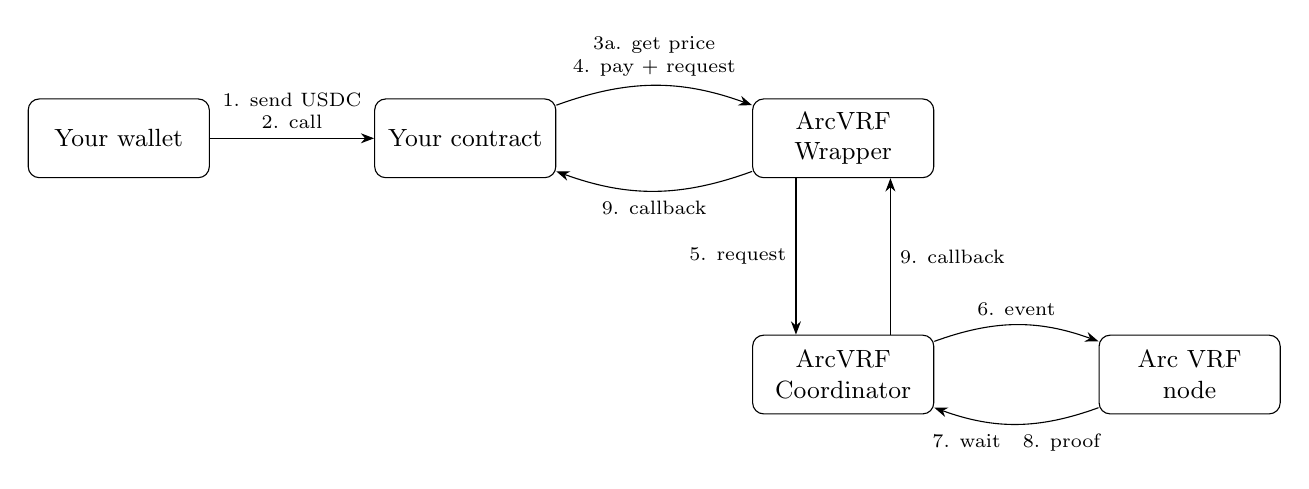
\begin{tikzpicture}[
  box/.style={draw,rounded corners,align=center,minimum width=2.3cm,minimum height=1cm,font=\small},
  lab/.style={font=\scriptsize,align=center},
  >=Stealth]
\node[box] (w) at (0,0) {Your wallet};
\node[box] (c) at (4.4,0) {Your contract};
\node[box] (wr) at (9.2,0) {ArcVRF\\Wrapper};
\node[box] (co) at (9.2,-3.0) {ArcVRF\\Coordinator};
\node[box] (n) at (13.6,-3.0) {Arc VRF\\node};
\draw[->] (w) -- node[lab,above]{1. send USDC\\2. call} (c);
\draw[->] (c) to[bend left=20] node[lab,above]{3a. get price\\4. pay + request} (wr);
\draw[->] (wr) to[bend left=20] node[lab,below]{9. callback} (c);
\draw[->] ([xshift=-6mm]wr.south) -- node[lab,left]{5. request} ([xshift=-6mm]co.north);
\draw[->] ([xshift=6mm]co.north) -- node[lab,right]{9. callback} ([xshift=6mm]wr.south);
\draw[->] (co) to[bend left=20] node[lab,above]{6. event} (n);
\draw[->] (n) to[bend left=20] node[lab,below]{7. wait\quad 8. proof} (co);
\end{tikzpicture}
\caption{Direct-funding flow (numbering follows Chainlink's diagram; step 3b is dropped on Arc).}
\end{figure}

\paragraph{The wrapper owns a subscription.} Chainlink's code says the wrapper's subscription ``is created and managed by an external account'' (VRFV2PlusWrapper.sol L184) \cite{clwrapper}. Live proof: Base Sepolia wrapper \code{0x7a1BaC17Ccc5b313516C5E16fb24f7659aA5ebed} (VRFV2PlusWrapper 1.0.0) owns subscription 7489\ldots6725 on coordinator \code{0x5C210eF41CD1a72de73bF76eC39637bB0d3d7BEE} and is its consumer (read 22 Nov 2026) \cite{bswrapper}. Your payments stay in the wrapper until the operator withdraws them; the operator keeps the wrapper's subscription funded.

\begin{itemize}
  \item Steps 3a to 6 happen in one transaction; the diagram draws them separately.
  \item The price is fixed when you request, using that transaction's gas price. Arc's smoothed base fee keeps it close to the real cost \cite{arcfee}.
  \item If your callback fails, the wrapper logs \code{WrapperFulfillmentFailed} instead of reverting, and there's no refund (L642--660).
\end{itemize}

\begin{deepdive}{direct-funding calls in the code}
{\small
\begin{tabularx}{\textwidth}{P{0.9cm}P{4.1cm}LP{1.9cm}}
\toprule
\# & Chainlink v2.5 call & What the code does & Arc VRF\\
\midrule
3a & \code{calculateRequestPriceNative(gas, numWords)} (Wrapper L392) & wrapperGasOverhead + (callbackGasLimit + coordinator overhead + per-word overhead) $\times$ (100 + premium)/100 + flat fee, at \code{tx.gasprice} (L433--455) & Same, in USDC\\
3b & \code{_calculateRequestPrice} + \code{_getFeedData} & Converts to LINK via price feed & Dropped\\
4 & \code{requestRandomWordsInNative{value}} (L560); LINK: \code{transferAndCall} $\to$ \code{onTokenTransfer} (L497) & Needs \code{msg.value} $\ge$ price and numWords $\le$ maxNumWords. Consumer base does 3a + 4 in one call: \code{requestRandomnessPayInNative} (ConsumerBase L76) & Native path only\\
5 & Wrapper $\to$ \code{requestRandomWords} with \code{SUBSCRIPTION_ID} (L574--582) & Gas limit = callback + EIP-150 overhead + wrapperGasOverhead; keyHash from the wrapper's config & Same\\
8 & \code{fulfillRandomWords(proof, rc, onlyPremium)} & Debits the wrapper's subscription & Same\\
9 & Wrapper \code{fulfillRandomWords} (L642--660) $\to$ \code{rawFulfillRandomWords} (ConsumerBase L104) & Exact-gas call to your contract & Same\\
Ops & \code{withdrawNative} (L611), \code{setConfig}, \code{enable}/\code{disable} & Operator collects fees and tunes overheads & Same\\
\bottomrule
\end{tabularx}}
\end{deepdive}

%-------------------------------------------------------------
\section{How the randomness is generated}
Two ingredients that no single party controls go into each result: the node's secret key, fixed in advance, and the hash of the block your request landed in, unknown before that block existed. Chainlink: it combines ``block data that is still unknown when the request is made with the oracle node's pre-committed private key'' \cite{cllaunch}.

\begin{figure}[ht]
\centering
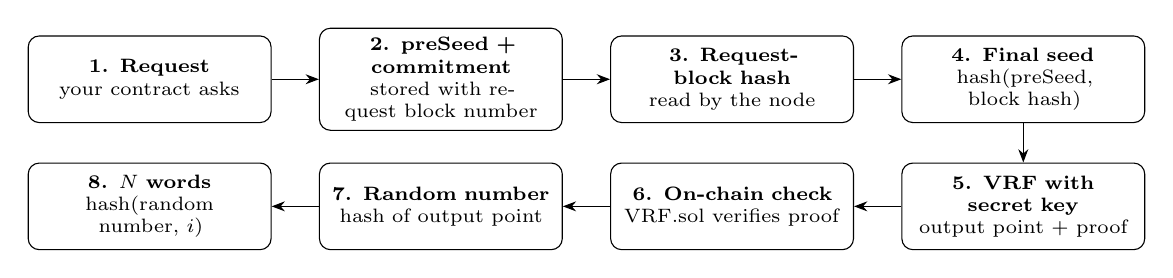
\begin{tikzpicture}[
  st/.style={draw,rounded corners,align=center,text width=2.85cm,minimum height=1.1cm,font=\scriptsize},
  >=Stealth, node distance=0.5cm and 0.6cm]
\node[st] (a) {\textbf{1. Request}\\your contract asks};
\node[st,right=of a] (b) {\textbf{2. preSeed + commitment}\\stored with request block number};
\node[st,right=of b] (c) {\textbf{3. Request-block hash}\\read by the node};
\node[st,right=of c] (d) {\textbf{4. Final seed}\\hash(preSeed, block hash)};
\node[st,below=of d] (e) {\textbf{5. VRF with secret key}\\output point + proof};
\node[st,left=of e] (f) {\textbf{6. On-chain check}\\VRF.sol verifies proof};
\node[st,left=of f] (g) {\textbf{7. Random number}\\hash of output point};
\node[st,left=of g] (h) {\textbf{8. $N$ words}\\hash(random number, $i$)};
\draw[->] (a)--(b); \draw[->] (b)--(c); \draw[->] (c)--(d); \draw[->] (d)--(e);
\draw[->] (e)--(f); \draw[->] (f)--(g); \draw[->] (g)--(h);
\end{tikzpicture}
\caption{From request to random words.}
\end{figure}

\begin{enumerate}[label=\textbf{\arabic*.}]
  \item \textbf{Request.} Your contract calls the coordinator.
  \item \textbf{preSeed and commitment.} The coordinator derives a preSeed from keyHash, your address, subscription ID and a counter, and stores a fingerprint of the request including the number of the block it's in.
  \item \textbf{Block hash.} The node reads the hash of that same request block. It is not a future block; the confirmation wait only delays the answer.
  \item \textbf{Final seed.} The node hashes preSeed together with that block hash.
  \item \textbf{VRF evaluation.} The node runs the seed through its secret key and gets an elliptic-curve point plus a proof.
  \item \textbf{On-chain verification.} The coordinator checks the public key is registered, rebuilds the final seed from on-chain data and verifies the proof. Any mismatch reverts.
  \item \textbf{Random number.} The coordinator computes it itself, as the hash of the proven point. The node never sends a bare number.
  \item \textbf{Expansion.} For $N$ numbers, the coordinator hashes the one random number with each index $i = 0, \ldots, N-1$. The expensive VRF runs once.
\end{enumerate}

\subsection{Who can cheat, and how}
{\small
\begin{tabularx}{\textwidth}{P{2.6cm}LL}
\toprule
Party & Can they pick or predict the result? & What they can still do\\
\midrule
Node (oracle) & Can't pick: only one output passes the proof check (``full uniqueness'', VRF.sol L41). It sees the result first. & Withhold the answer. Visible on-chain; apps must not re-request \cite{clsecurity}.\\
Validators & Can't predict: they know the block hash but not the secret key. & On chains with reorgs, rewrite history to re-roll, without knowing the new result. Arc has no reorgs.\\
Validators + stolen key & Yes. Chainlink: an adversary with the secret key and the ability to construct blocks ``could strongly bias the result'' \cite{clvrf}. & Key security now; more than one operator later.\\
You (the caller) & Can't simulate: without the secret key nobody can compute the output, even after the block hash is public. & Nothing, if your app follows the security guidance.\\
\bottomrule
\end{tabularx}}

\paragraph{Arc with 0 confirmations.} Chainlink uses confirmations so a rewrite can't move a request into a different block and re-roll it \cite{clsecurity}. Arc finalizes on inclusion and its BFT consensus makes reorgs impossible \cite{arcconsensus}. So with 0 confirmations, Arc VRF's guarantee rests on Arc's BFT finality (a permissioned validator set) plus the node's pre-registered key.

\subsection{Common explanations, checked against the code}
{\small
\begin{tabularx}{\textwidth}{P{3.6cm}P{1.9cm}L}
\toprule
Claim & Verdict & What the code and docs say\\
\midrule
The node waits for a future block and uses its hash & \textbf{Wrong} & It's the request block's hash. The commitment stores \code{_getBlockNumber()} at request time (Coordinator L302--305); fulfilment uses \code{_getBlockhash(rc.blockNum)} (L393). Confirmations only delay the answer.\\
The oracle publishes PK on-chain, shown by keyHash & Partly & The coordinator owner registers it (\code{registerProvingKey}, onlyOwner, L109--120). Only keyHash $=$ \code{keccak256(abi.encode(pk))} is stored (L151--155); the full key is in that transaction's data and in every proof.\\
The oracle sends the number and the proof & Partly & It sends the proof and request data; the contract derives the number: \code{keccak256(abi.encode(3, gamma))} (VRF.sol L592--600).\\
The coordinator verifies the proof on-chain & Correct & \code{_getRandomnessFromProof} (L369--405) $\to$ \code{VRF._randomValueFromVRFProof}, which reverts on failure.\\
The oracle can't choose, only withhold & Correct & Uniqueness (VRF.sol L41). Residual risks: withholding; key theft plus block building.\\
Validators can't predict without SK & Correct & They can still re-roll on chains with reorgs \cite{clsecurity}. Arc has none.\\
The caller can't simulate because the block isn't final yet & Right result, wrong reason & The real reason is the secret key: once the request is in a block, its hash is public, yet only the key holder can compute the output.\\
numWords expands one output with a counter & Correct & \code{randomWords[i] = keccak256(abi.encode(randomness, i))} (L489--493), on-chain.\\
``Goldberg's VRF over secp256k1'' & Close & VRF.sol follows Goldberg et al., draft-irtf-cfrg-vrf-05 \cite{vrfdraft}, with proofs in ePrint 2017/099 \cite{eprint}, on secp256k1 with Keccak. Not byte-compatible with the final RFC 9381 \cite{rfc9381}.\\
\bottomrule
\end{tabularx}}

\noindent Sources used: Chainlink code and docs, RFC 9381 and Chainlink's 2020 launch post. Secondary articles (speedrunethereum, dev.to, webisoft) were not relied on.

\begin{deepdive}{exact formulas}
Let $\mathrm{H}$ denote \code{keccak256} and $\|$ denote ABI encoding of the listed values. At request time (VRFCoordinatorV2\_5.sol L322--330, L302--305):
\begin{align*}
\mathit{preSeed} &= \mathrm{H}\big(\mathit{keyHash} \,\|\, \mathit{sender} \,\|\, \mathit{subId} \,\|\, \mathit{nonce}\big)\\
\mathit{requestId} &= \mathrm{H}\big(\mathit{keyHash} \,\|\, \mathit{preSeed}\big)\\
\mathit{commitment}[\mathit{requestId}] &= \mathrm{H}\big(\mathit{requestId} \,\|\, b_{\text{req}} \,\|\, \mathit{subId} \,\|\, \mathit{callbackGasLimit}\\
&\qquad\quad \,\|\, \mathit{numWords} \,\|\, \mathit{sender} \,\|\, \mathit{extraArgs}\big)
\end{align*}
where $b_{\text{req}}$ is the request block number. At fulfilment time (L369--405):
\begin{align*}
\mathit{keyHash} &= \mathrm{H}(\mathit{pk}) \quad\text{(must be registered; \code{hashOfKey}, L151)}\\
\mathit{actualSeed} &= \mathrm{H}_{\text{packed}}\big(\mathit{preSeed} \,\|\, \mathrm{blockhash}(b_{\text{req}})\big)\\
\mathit{randomness} &= \mathrm{H}\big(3 \,\|\, \Gamma\big) \quad\text{(VRF.sol L592--600, after the proof verifies)}\\
\mathit{randomWords}[i] &= \mathrm{H}\big(\mathit{randomness} \,\|\, i\big), \qquad i = 0, \ldots, \mathit{numWords}-1 \quad\text{(L489--493)}
\end{align*}
The same in code:
\begin{lstlisting}[language=Solidity]
// Request time (VRFCoordinatorV2_5.sol L322-330, L302-305)
preSeed   = keccak256(abi.encode(keyHash, sender, subId, nonce))
requestId = keccak256(abi.encode(keyHash, preSeed))
commitment[requestId] = keccak256(abi.encode(requestId, block.number /* request block */,
                          subId, callbackGasLimit, numWords, sender, extraArgs))

// Fulfilment time (L369-405)
keyHash    = keccak256(abi.encode(proof.pk))              // must be registered (hashOfKey, L151)
requestId  = keccak256(abi.encode(keyHash, proof.seed))   // proof.seed == preSeed
blockHash  = blockhash(rc.blockNum)                       // the REQUEST block; BlockhashStore fallback
actualSeed = keccak256(abi.encodePacked(proof.seed, blockHash))
randomness = keccak256(abi.encode(3, proof.gamma))        // VRF.sol L592-600, after proof verifies

// Expansion (L489-493)
randomWords[i] = keccak256(abi.encode(randomness, i))     // i = 0 .. numWords-1
\end{lstlisting}
\begin{itemize}
  \item Why the block hash is needed: preSeed is predictable (it uses a counter), so without it the node could compute outputs before requests arrive \cite{cllaunch}.
  \item VRF.sol deviates from the IETF draft on purpose: secp256k1 so \code{ecrecover} gives cheap scalar multiplication, Keccak instead of SHA-256, its own hash-to-curve, address of $u$ in the challenge (VRF.sol L1--130) \cite{clvrfsol}. Arc VRF keeps that scheme.
  \item Arc supports the precompiles needed: \code{ecrecover} (0x01) and modexp (0x05) returned correct test vectors on Arc mainnet and testnet (22 Nov 2026).
  \item RFC 9381 \S3.4: anyone holding the secret key can compute outputs, so the key must be generated honestly and kept secret \cite{rfc9381}.
\end{itemize}
\end{deepdive}

%-------------------------------------------------------------
\section{Request parameters}
Checked against \code{VRFV2PlusClient.sol}, the coordinator, the wrapper and Chainlink's docs \cite{clclient,clmigv2,clgetsub,clgetdf}.

\subsection{Subscription method: \texorpdfstring{\texttt{VRFV2PlusClient.RandomWordsRequest}}{VRFV2PlusClient.RandomWordsRequest}}
{\small
\begin{tabularx}{\textwidth}{P{2.9cm}P{1.3cm}LP{2.4cm}}
\toprule
Field & Type & Chainlink meaning & Arc VRF\\
\midrule
\code{keyHash} & bytes32 & Picks the node's key and the gas lane (max gas price). Not checked at request time; an unknown keyHash is simply never fulfilled (Coordinator L294--296) & Same; one or two Arc lanes\\
\code{subId} & uint256 & Subscription that pays. Was uint64 in v2 \cite{clmigv2} & Same\\
\code{requestConfirmations} & uint16 & Blocks the node waits; between the coordinator minimum and 200 & Minimum 0\\
\code{callbackGasLimit} & uint32 & Gas for your callback; reverts if above maxGasLimit & Same; limit measured on Arc\\
\code{numWords} & uint32 & How many numbers; max 500 & Same\\
\code{extraArgs} & bytes & \code{_argsToBytes(ExtraArgsV1({nativePayment}))}: 4-byte version tag + options. Empty means LINK & Kept (see decision)\\
\bottomrule
\end{tabularx}}

\begin{lstlisting}[language=Solidity]
VRFV2PlusClient.RandomWordsRequest({
  keyHash: KEY_HASH,                 // gas lane on Arc
  subId: s_subId,                    // uint256
  requestConfirmations: 0,           // Arc minimum
  callbackGasLimit: 200_000,
  numWords: 1,
  extraArgs: VRFV2PlusClient._argsToBytes(
    VRFV2PlusClient.ExtraArgsV1({nativePayment: true}) // Arc: must be true or empty
  )
})
\end{lstlisting}

\subsection{Direct funding: wrapper consumer}
{\small
\begin{tabularx}{\textwidth}{P{3.0cm}LP{2.8cm}}
\toprule
Field & Chainlink meaning & Arc VRF\\
\midrule
\code{callbackGasLimit} & At most maxGasLimit minus wrapperGasOverhead \cite{cldf} & Same\\
\code{requestConfirmations} & Blocks the node waits & Minimum 0\\
\code{numWords} & At most the wrapper's maxNumWords (10 on Base Sepolia) & Same; start at 10\\
\code{extraArgs} & nativePayment true for the native path, false or empty for LINK (\code{checkPaymentMode}, Wrapper L533) & Kept (see decision)\\
\code{keyHash} & Not passed per call; set on the wrapper (\code{s_keyHash} via \code{setConfig}) & Same\\
\bottomrule
\end{tabularx}}

\paragraph{Function names.} \code{requestRandomness} (LINK) and \code{requestRandomnessPayInNative} (native) are internal helpers in \code{VRFV2PlusWrapperConsumerBase} (L62, L76) \cite{clwrapperbase}, not functions on the wrapper. The wrapper's own entry points are \code{onTokenTransfer} (LINK) and \code{requestRandomWordsInNative} (native). Arc VRF keeps only \code{requestRandomnessPayInNative}.

\paragraph{Decision on \texttt{extraArgs} [Design choice].} Keep the \code{extraArgs} field and Chainlink's versioned encoding (\code{EXTRA_ARGS_V1_TAG} + \code{ExtraArgsV1}). Accept empty or \code{nativePayment: true}; revert on \code{nativePayment: false} with a clear error. Why: Chainlink consumer code ports unchanged, the version tag leaves room for future options, and nobody can silently believe they're paying in LINK. This differs from Chainlink, where empty means LINK.

%-------------------------------------------------------------
\section{Arc-specific design}
\begin{itemize}
  \item \textbf{USDC only.} Arc's native gas token is USDC with 18 decimals, so fees are already in USDC and no price feed is needed \cite{arcevm}. LINK payment, the LINK feed and L2 fee code are removed.
  \item \textbf{Confirmations default to 0.} Arc: ``Finality is deterministic and instant. Transactions finalize on inclusion'' \cite{arcfinality}. The field stays, so apps can ask for more.
  \item \textbf{Older block hashes.} Arc blocks are about 0.51\,s apart, so the usual 256-block window is about 2 minutes. Arc VRF overrides \code{_getBlockhash} (CL L642, built to be overridden) to fall back to EIP-2935 history at \code{0x0000F90827F1C53a10cb7A02335B175320002935} (served $n-8000$, failed at $n-9000$, measured), then BlockhashStore.
  \item \textbf{Gas floor.} The node sets maxFeePerGas $\ge 20$\,gwei; lower is ``silently dropped by the mempool'' \cite{arcevm}.
  \item \textbf{USDC sends can fail.} Arc's blocklist and zero-address rules can revert a native transfer, so withdrawals stay pull-based and never block cancellation.
  \item \textbf{Indexing.} Arc emits EIP-7708 \code{Transfer} logs for native moves; don't double-count funding \cite{arcindex}.
  \item \textbf{Keys [Recommendation].} VRF proving key in an HSM, KMS or dedicated encrypted keystore, separate from the transaction-sending key, as Chainlink does on Base Sepolia.
\end{itemize}

%-------------------------------------------------------------
\section{Security}
{\small
\begin{tabularx}{\textwidth}{P{4.0cm}LL}
\toprule
Threat & Chainlink & Arc VRF\\
\midrule
Node picks a favourable output & Impossible: uniqueness + on-chain proof & Same\\
Node withholds & Visible on-chain & One operator can withhold; second operator later\\
Node precomputes outputs & Request block hash mixed in & Same\\
Reorg re-roll & requestConfirmations & No reorgs on Arc, so 0\\
Validators + stolen key & Can strongly bias & Same risk; Arc validators are a permissioned set\\
Your callback reverts & Not retried, still charged & Same; SDK guidance\\
Wrapper subscription runs dry & Operator tops up & Alerts; optional auto top-up\\
USDC refund fails & n/a & Pull-based withdrawals\\
Block hash too old & BlockhashStore & EIP-2935 first\\
\bottomrule
\end{tabularx}}

\subsection*{Limits and trust assumptions}
\begin{itemize}
  \item One operator and one key at launch: it controls liveness, sees outputs first and can withhold.
  \item The coordinator owner can change fees, settings and keys, as in Chainlink.
  \item Arc's validators are a permissioned proof-of-authority set; Arc VRF inherits Arc's liveness and censorship properties.
  \item No staking or slashing. Don't call it decentralised until there is more than one independent operator.
\end{itemize}

%-------------------------------------------------------------
\section{Economics}
Fees are gas cost plus a percentage premium plus an optional flat fee, all in USDC. Arc's base fee is smoothed and priced in USDC \cite{arcfee}, so fees stay stable in dollars.

\subsection{Fee formulas}
Let $g$ be the gas price in wei, $p$ the premium percentage and $f$ the flat fee in parts per million (PPM). Amounts are in the native unit's smallest denomination (USDC with 18 decimals on Arc).

\paragraph{Subscription, charged after fulfilment} (Coordinator L559--580):
\[
\mathit{payment} = \frac{g \cdot \big(\mathit{gasAfterPaymentCalculation} + \mathit{gasUsed}\big)\cdot(100+p)}{100} + 10^{12}\cdot f
\]

\paragraph{Direct funding, quoted at request} (Wrapper L433--455):
\begin{multline*}
\mathit{price} = g\cdot \mathit{wrapperGasOverhead}\\
+ \frac{g\cdot\big(\mathit{callbackGasLimit} + \mathit{coordOverheadNative} + \mathit{numWords}\cdot \mathit{perWord}\big)\cdot(100+p)}{100} + 10^{12}\cdot f
\end{multline*}

\paragraph{Maximum cost a subscription must cover} (Chainlink's formula \cite{clsub}):
\[
\mathit{maxCost} = \frac{g_{\max}\cdot\big(200{,}000 + \mathit{callbackGasLimit}\big)\cdot(100+p)}{100}
\]

\subsection{Worked example (direct funding)}
Using the live Base Sepolia wrapper settings (wrapperGasOverhead 13{,}400; coordinator native overhead 128{,}500; 435 per word; premium 60\%; flat fee 0) at Arc's current 20\,gwei base fee, with callbackGasLimit $=100{,}000$ and numWords $=1$:
\begin{align*}
g\cdot \mathit{wrapperGasOverhead} &= 20\times10^{9}\times 13{,}400 = 2.68\times10^{14}\\
g\cdot(100{,}000+128{,}500+435)\cdot\tfrac{160}{100} &= 20\times10^{9}\times 228{,}935\times 1.6 = 7.32592\times10^{15}\\
\mathit{price} &= 7.59392\times10^{15}\ \text{wei} = 0.00759392
\end{align*}
That is 0.007594 per request, matching that wrapper's own \code{estimateRequestPriceNative(100000, 1, 20 gwei)} $=$ 0.00759392 ETH (read 22 Nov 2026) \cite{bswrapper}. On Arc the unit is USDC. Arc VRF's real overheads must be measured on Arc.

\subsection{Worked example (subscription) [estimate]}
The Base Sepolia fulfilment billed about 214{,}587 gas. At 20\,gwei with a 50\% premium that is about 0.0064 USDC per request. This is an estimate, not a measurement on Arc.

%-------------------------------------------------------------
\section{Live reference: Chainlink on Base Sepolia}
\code{0xd427...5a5b} \cite{bsbatch} is BatchVRFCoordinatorV2Plus, a helper the Chainlink node uses to submit answers; it forwards to the real coordinator \code{0x5C210eF41CD1a72de73bF76eC39637bB0d3d7BEE} \cite{bscoord}. The fulfilment transaction \cite{bsfulfil} is the fulfilment, not the request.

\begin{enumerate}[label=\textbf{\arabic*.}]
  \item \textbf{Subscription set up (25 Sep 2026, IST):} created, funded with ETH and 25 LINK, HiLoGame added.
  \item \textbf{Request (28 Sep, 02:39:14 IST, block 47,387,533):} HiLoGame calls \code{requestRandomWords}: 3 confirmations, 500,000 callback gas, 1 word, LINK payment.
  \item \textbf{Fulfil (02:39:22 IST, block 47,387,537):} 4 blocks (8\,s) later; 204,839 gas used.
  \item \textbf{Callback:} previous ball 4, new ball 14, outcome Hi.
  \item \textbf{Billing:} 0.000386 LINK.
\end{enumerate}
Re-checked locally: the keyHash is the hash of the proof's public key, the requestId matches, the random output is the hash of the proof's point, and word 0 maps to ball 14 exactly as HiLoGame emitted.

\begin{deepdive}{settings and transactions}
\begin{itemize}
  \item Coordinator VRFCoordinatorV2\_5\_Optimism (MIT); min confirmations 0 (max 200); maxGasLimit 2,500,000; premium 60\% native / 50\% LINK, flat fee 0; max 100 consumers, 500 words; key hash (30\,gwei lane) \code{0x9e1344a1...bf71}.
  \item Wrapper VRFV2PlusWrapper 1.0.0 \code{0x7a1BaC17Ccc5b313516C5E16fb24f7659aA5ebed}; overheads 13,400 / 128,500 / 435; maxNumWords 10.
  \item Consumer HiLoGame \code{0x5FA7D3D07059d98e33ebF833306cE1014eA852Bd} \cite{bshilo}.
\end{itemize}
{\small
\begin{tabularx}{\textwidth}{P{3.0cm}P{3.2cm}L}
\toprule
When (IST) & Event & Transaction\\
\midrule
25 Sep 2026 01:42:40 & SubscriptionCreated & \url{https://sepolia.basescan.org/tx/0xc8319d491862c5bb891db190d88ffcf7f485fd8704f29dd79aa7e47c1b71b18a}\\
25 Sep 01:48:44 & ConsumerAdded (HiLoGame) & \url{https://sepolia.basescan.org/tx/0x370b81bc47b5b5326e2a652818c905d9edadd6913531e8eb450244a314653252}\\
25 Sep 02:36:14 & Funded 25 LINK & \url{https://sepolia.basescan.org/tx/0xd75157b743dcbc2173d8536d072fa3b8dc95acc73662dac250373850fc2ca858}\\
28 Sep 02:39:14 & Request & \url{https://sepolia.basescan.org/tx/0x37698ef8c02b356fc49eb04a59363c68ef8b6513f6aeb80f7772b416af1d9ed3}\\
28 Sep 02:39:22 & Fulfilment & \url{https://sepolia.basescan.org/tx/0x9bdf053b40482ef98639ba5fe18172f7f7dce86bb6234bfcca85488e91519097}\\
\bottomrule
\end{tabularx}}
\end{deepdive}

%-------------------------------------------------------------
\section{Build plan and milestones}
\begin{description}[leftmargin=1em,style=nextline]
  \item[Contracts] Fork Chainlink v2.5 at e162754, keeping MIT notices. \code{ArcVRFCoordinator} (coordinator + subscriptions, USDC only, EIP-2935 fallback), \code{ArcVRFWrapper} (native path only), \code{ArcVRFConsumerBase}, \code{ArcVRFWrapperConsumerBase}, \code{VRF.sol} unchanged, batch helper, \code{BlockhashStore}.
  \item[Node] Listener, proof generator (port of Chainlink's Go proof code), transaction manager with 20\,gwei floor, balance check, metrics. Go or TypeScript.
  \item[Indexer] Subscription, consumer, funding, request and fulfilment events, de-duplicating Arc's EIP-7708 logs.
  \item[Dashboard] Wallet connect on 5042002 / 5042. Subscription manager: create, fund, consumers, history, transfer, cancel. Direct funding: live fee calculator (\code{estimateRequestPriceNative}, \code{getConfig}), wrapper settings, request history, docs.
  \item[SDK and docs] Both consumer bases, two Foundry templates, TypeScript helpers for subscription calls and price quotes.
  \item[Wrapper operations] Create and fund its subscription, add it as consumer, set config, balance alerts, withdraw fees.
  \item[Tooling] Arc Foundry; stock anvil can't reproduce Arc behaviour \cite{arcevm}.
\end{description}

\subsection{Milestones}
Durations are estimates.
\begin{description}[leftmargin=1em,style=nextline]
  \item[M0 (week 1)] Fork coordinator and wrapper, strip LINK, compile with Arc Foundry, unit tests green for both methods.
  \item[M1 (weeks 2--3)] Arc testnet (5042002): deploy both, set up the wrapper's subscription, node v0, dashboard v0 with subscription manager and fee calculator; port HiLoGame plus a direct-funding sample.
  \item[M2 (weeks 4--5)] Batch fulfilment, EIP-2935 fallback, monitoring, measure Arc gas overheads, load-test both methods.
  \item[M3 (weeks 6--8)] External audit of coordinator and wrapper, key ceremony, license legal review.
  \item[M4] Arc mainnet (5042) beta of both methods with caps and a public status page; then a second operator.
\end{description}

\subsection{Test plan}
\begin{itemize}
  \item Unit tests for every call and revert in both flows.
  \item Node vs VRF.sol proof tests on random seeds.
  \item Replay the Base Sepolia request and fulfilment as fixtures.
  \item Wrapper: price matches formula; underpaying and too many words revert; failing callback emits \code{WrapperFulfillmentFailed}.
  \item Invariants: balances add up; nothing fulfilled twice.
  \item Failure cases: out of gas, blocked withdrawal, request older than 8,191 blocks.
\end{itemize}

\subsection{Audit checklist}
\begin{itemize}
  \item Commitment check, coordinator-only callback, exact-gas call, reentrancy lock.
  \item \code{extraArgs} rules (empty or native only).
  \item USDC send failures under Arc rules.
  \item Owner powers behind a multisig or timelock.
  \item Key storage, rotation and removal runbook.
  \item Node idempotency, de-duplication, RPC failover.
\end{itemize}

%-------------------------------------------------------------
\section{Open questions}
\begin{enumerate}
  \item Go or TypeScript for the node?
  \item Premium \% and flat fee for each method? Chainlink's Base Sepolia wrapper charges 60\%.
  \item One operator at launch, or two?
  \item Should the wrapper top up its own subscription automatically from fees? Chainlink's doesn't.
  \item Also accept ERC-20 USDC deposits (6 decimals)? Arc warns against mixing them with native amounts.
  \item Gas lane maximums on Arc.
  \item Does Arc's block header format work with \code{BlockhashStore.storeVerifyHeader}? \textbf{[Unverified]}
  \item Do consumers in Arc's privacy sector work, given events are off by default \cite{arcprivacy}? \textbf{[Unverified]}
  \item Legal review of package-level BUSL vs per-file MIT.
\end{enumerate}

%-------------------------------------------------------------
\section{Comparables and unverified claims}
{\small
\begin{tabularx}{\textwidth}{P{2.6cm}LP{2.6cm}P{1.2cm}}
\toprule
Service & How it works & On Arc? & Source\\
\midrule
Chainlink VRF v2.5 & One key per node, on-chain proof & No & \cite{clnetworks}\\
D20DAO & drand + VRF, pay per request in USDC & Yes, per its docs & \cite{d20dao}\\
Pyth Entropy & Two-party commit/reveal & Not in its chain lists & \cite{pyth}\\
Gelato VRF & Nodes relay drand & Not checked & \cite{gelato}\\
Supra dVRF & Threshold BLS & Not checked & \cite{supra}\\
API3 QRNG & Discontinued from 1 Jan 2025 & n/a & \cite{api3}\\
\bottomrule
\end{tabularx}}

\medskip
\noindent\textbf{Not verified:} whether Gelato VRF or Supra dVRF run on Arc; D20DAO's security claims; a search summary saying Pyth Entropy is on Arc (the cited note was about other Pyth products); the Arc per-request cost (estimate only).

%-------------------------------------------------------------
\begin{thebibliography}{99}
\small
\bibitem{clvrf} Chainlink. \emph{Chainlink VRF} (includes the v1/v2 shutdown notice). \url{https://docs.chain.link/vrf}
\bibitem{clproduct} Chainlink. \emph{Chainlink VRF product page}. \url{https://chain.link/vrf}
\bibitem{cledu1} Chainlink. \emph{What is a verifiable random function}. \url{https://chain.link/education-hub/verifiable-random-function-vrf}
\bibitem{cledu2} Chainlink. \emph{Randomness in Web3}. \url{https://chain.link/education-hub/randomness-web3}
\bibitem{clsub} Chainlink. \emph{VRF v2.5 subscription method}. \url{https://docs.chain.link/vrf/v2-5/overview/subscription}
\bibitem{cldf} Chainlink. \emph{VRF v2.5 direct funding method}. \url{https://docs.chain.link/vrf/v2-5/overview/direct-funding}
\bibitem{clgetsub} Chainlink. \emph{Get a random number (subscription)}. \url{https://docs.chain.link/vrf/v2-5/subscription/get-a-random-number}
\bibitem{clgetdf} Chainlink. \emph{Get a random number (direct funding)}. \url{https://docs.chain.link/vrf/v2-5/direct-funding/get-a-random-number}
\bibitem{clmigv2} Chainlink. \emph{Migrating from VRF v2}. \url{https://docs.chain.link/vrf/v2-5/migration-from-v2}
\bibitem{clmigv1} Chainlink. \emph{Migrating from VRF v1}. \url{https://docs.chain.link/vrf/v2-5/migration-from-v1}
\bibitem{clbilling} Chainlink. \emph{VRF v2.5 billing}. \url{https://docs.chain.link/vrf/v2-5/billing}
\bibitem{clsecurity} Chainlink. \emph{VRF security considerations}. \url{https://docs.chain.link/vrf/v2-5/security}
\bibitem{clnetworks} Chainlink. \emph{VRF supported networks}. \url{https://docs.chain.link/vrf/v2-5/supported-networks}
\bibitem{cllaunch} Chainlink (2020). \emph{Chainlink VRF: On-chain verifiable randomness}. \url{https://blog.chain.link/chainlink-vrf-on-chain-verifiable-randomness/}
\bibitem{clcode} smartcontractkit/chainlink-evm, commit e162754, \code{contracts/src/v0.8/vrf/}. \url{https://github.com/smartcontractkit/chainlink-evm/blob/e162754ee3348c8c44a691669f710a06761dd67f/contracts/src/v0.8/vrf/}
\bibitem{clcoordinator} \code{VRFCoordinatorV2_5.sol}. \url{https://github.com/smartcontractkit/chainlink-evm/blob/e162754ee3348c8c44a691669f710a06761dd67f/contracts/src/v0.8/vrf/VRFCoordinatorV2_5.sol}
\bibitem{clsubapi} \code{SubscriptionAPI.sol}. \url{https://github.com/smartcontractkit/chainlink-evm/blob/e162754ee3348c8c44a691669f710a06761dd67f/contracts/src/v0.8/vrf/SubscriptionAPI.sol}
\bibitem{clvrfsol} \code{VRF.sol}. \url{https://github.com/smartcontractkit/chainlink-evm/blob/e162754ee3348c8c44a691669f710a06761dd67f/contracts/src/v0.8/vrf/VRF.sol}
\bibitem{clwrapper} \code{VRFV2PlusWrapper.sol}. \url{https://github.com/smartcontractkit/chainlink-evm/blob/e162754ee3348c8c44a691669f710a06761dd67f/contracts/src/v0.8/vrf/VRFV2PlusWrapper.sol}
\bibitem{clwrapperbase} \code{VRFV2PlusWrapperConsumerBase.sol}. \url{https://github.com/smartcontractkit/chainlink-evm/blob/e162754ee3348c8c44a691669f710a06761dd67f/contracts/src/v0.8/vrf/VRFV2PlusWrapperConsumerBase.sol}
\bibitem{clclient} \code{VRFV2PlusClient.sol}. \url{https://github.com/smartcontractkit/chainlink-evm/blob/e162754ee3348c8c44a691669f710a06761dd67f/contracts/src/v0.8/vrf/libraries/VRFV2PlusClient.sol}
\bibitem{clconsumer} \code{VRFConsumerBaseV2Plus.sol}. \url{https://github.com/smartcontractkit/chainlink-evm/blob/e162754ee3348c8c44a691669f710a06761dd67f/contracts/src/v0.8/vrf/VRFConsumerBaseV2Plus.sol}
\bibitem{clbhs} \code{BlockhashStore.sol}. \url{https://github.com/smartcontractkit/chainlink-evm/blob/e162754ee3348c8c44a691669f710a06761dd67f/contracts/src/v0.8/vrf/BlockhashStore.sol}
\bibitem{cllicense} chainlink-evm LICENSE. \url{https://github.com/smartcontractkit/chainlink-evm/blob/develop/LICENSE}
\bibitem{clnpm} \code{@chainlink/contracts} on npm. \url{https://www.npmjs.com/package/@chainlink/contracts}
\bibitem{rfc9381} S.~Goldberg, L.~Reyzin, D.~Papadopoulos, J.~V\v{c}el\'ak. \emph{RFC 9381: Verifiable Random Functions (VRFs)}, IETF, 2023. \url{https://www.rfc-editor.org/rfc/rfc9381}
\bibitem{vrfdraft} S.~Goldberg et al. \emph{draft-irtf-cfrg-vrf-05}, IETF, 2019. \url{https://datatracker.ietf.org/doc/html/draft-irtf-cfrg-vrf-05}
\bibitem{eprint} D.~Papadopoulos et al. \emph{ePrint 2017/099}. \url{https://eprint.iacr.org/2017/099.pdf}
\bibitem{arcevm} Arc. \emph{EVM differences}. \url{https://docs.arc.io/arc/references/evm-differences.md}
\bibitem{arcrpc} Arc. \emph{RPC endpoints and chain IDs}. \url{https://docs.arc.io/arc/references/rpc-endpoints.md}
\bibitem{arcfinality} Arc. \emph{Deterministic finality}. \url{https://docs.arc.io/arc/concepts/deterministic-finality.md}
\bibitem{arcconsensus} Arc. \emph{Consensus layer}. \url{https://docs.arc.io/arc/concepts/consensus-layer.md}
\bibitem{arcfee} Arc. \emph{Stable fee design}. \url{https://docs.arc.io/arc/concepts/stable-fee-design.md}
\bibitem{arcprivacy} Arc. \emph{Opt-in privacy}. \url{https://docs.arc.io/arc/concepts/opt-in-privacy.md}
\bibitem{arcoracles} Arc. \emph{Oracles}. \url{https://docs.arc.io/arc/tools/oracles.md}
\bibitem{arcindex} Arc. \emph{Indexing events}. \url{https://docs.arc.io/integrate/infrastructure/indexing-events.md}
\bibitem{bsbatch} BatchVRFCoordinatorV2Plus on Base Sepolia. \url{https://sepolia.basescan.org/address/0xd427446551a93f4686799edeca33bbb741115a5b#code}
\bibitem{bscoord} VRF coordinator on Base Sepolia. \url{https://sepolia.basescan.org/address/0x5C210eF41CD1a72de73bF76eC39637bB0d3d7BEE}
\bibitem{bswrapper} VRF v2.5 wrapper on Base Sepolia. \url{https://sepolia.basescan.org/address/0x7a1BaC17Ccc5b313516C5E16fb24f7659aA5ebed}
\bibitem{bshilo} HiLoGame consumer on Base Sepolia. \url{https://sepolia.basescan.org/address/0x5FA7D3D07059d98e33ebF833306cE1014eA852Bd}
\bibitem{bsfulfil} Fulfilment transaction on Base Sepolia. \url{https://sepolia.basescan.org/tx/0x9bdf053b40482ef98639ba5fe18172f7f7dce86bb6234bfcca85488e91519097}
\bibitem{d20dao} D20DAO documentation. \url{https://d20dao.org/llms-full.txt}
\bibitem{pyth} Pyth. \emph{Entropy protocol design}. \url{https://docs.pyth.network/entropy/protocol-design}
\bibitem{supra} Supra. \emph{dVRF architecture guide}. \url{https://docs.supra.com/dvrf/learn-supra-dvrf/supra-dvrf-architecture-guide}
\bibitem{gelato} Arbitrum docs. \emph{Gelato VRF}. \url{https://docs.arbitrum.io/third-party-docs/Gelato/gelato-vrf}
\bibitem{api3} Cryptowisser. \emph{API3 will no longer support the QRNG service}. \url{https://www.cryptowisser.com/news/api3-will-no-longer-support-the-qrng-service/}
\bibitem{repoarc} H.~Malik. \code{arc-vrf} repository. \url{https://github.com/HimanshuM685/arc-vrf}
\bibitem{repohilo} H.~Malik. \code{rack-up-hi-lo} repository. \url{https://github.com/HimanshuM685/rack-up-hi-lo}
\end{thebibliography}

\nocite{clproduct,cledu1,cledu2,clbilling,clcoordinator,clsubapi,clconsumer,clbhs,repohilo}

\end{document}
